\documentclass{beamer}
\usepackage[utf8]{inputenc}
\usepackage{amssymb}
\usepackage{tikz}
\usetikzlibrary{positioning}

\tikzset{set/.style={draw,circle,inner sep=0pt,align=center}}

\usepackage{appendixnumberbeamer}

\usetheme[sectionpage=progressbar,subsectionpage=progressbar,numbering=fraction,
          progressbar=foot]{metropolis}

\title{Cloud \& Big Data}
\subtitle{Elasticity in Cloud Computing}

\date{\today}
\author{%
  Simon Bihel, \url{simon.bihel@ens-rennes.fr} \\
  Rémi Hutin, \url{remi.hutin@ens-rennes.fr}
}
\institute{%
  University of Rennes I \\
  École normale supérieure de Rennes
}

\begin{document}

\maketitle

\begin{frame}{Table of contents}
  \setbeamertemplate{section in toc}[sections numbered]
  \tableofcontents[hideallsubsections]
\end{frame}


\section{Elasticity: Definition and Differentiation}
\begin{frame}
  \frametitle{What It Is Not~\cite{herbst2013elasticity}}
  \begin{description}
    \parbox{\linewidth}{%
    \item[Scalability] Sustain increasing workloads with adequate performance.
    \item[Efficiency] Amount of resources consumed for a given amount of work.
    }
  \end{description}
\end{frame}

\begin{frame}
  \frametitle{}
  \centering
  \Large\textbf{Elasticity} $\neq$ \textbf{Scalability}

  \visible<2->{It's more than that. That's the selling point.}
\end{frame}

\begin{frame}
\begin{figure}
\tikzstyle{every path}=[line width=1pt, color=orange, text=white]
\def\firstcircle{(-2.85,0) circle (1.5cm)}
\def\secondcircle{(0,2.85) circle (1.5cm)}
\def\thirdcircle{(2.85,0) circle (1.5cm)}
\begin{tikzpicture}
    \begin{scope}[shift={(3cm,-5cm)}]
        \fill[black!60] \firstcircle;
        \fill[black!60] \secondcircle;
        \fill[black!60] \thirdcircle;
        \draw \firstcircle node {\Large Speed};
        \draw \secondcircle node {\Large Scalability};
        \draw \thirdcircle node {\Large Precision};
    \end{scope}
\end{tikzpicture}
\end{figure}
\end{frame}

\begin{frame}
  \frametitle{Example of matching demand~\cite{herbst2013elasticity}}
  \begin{figure}
    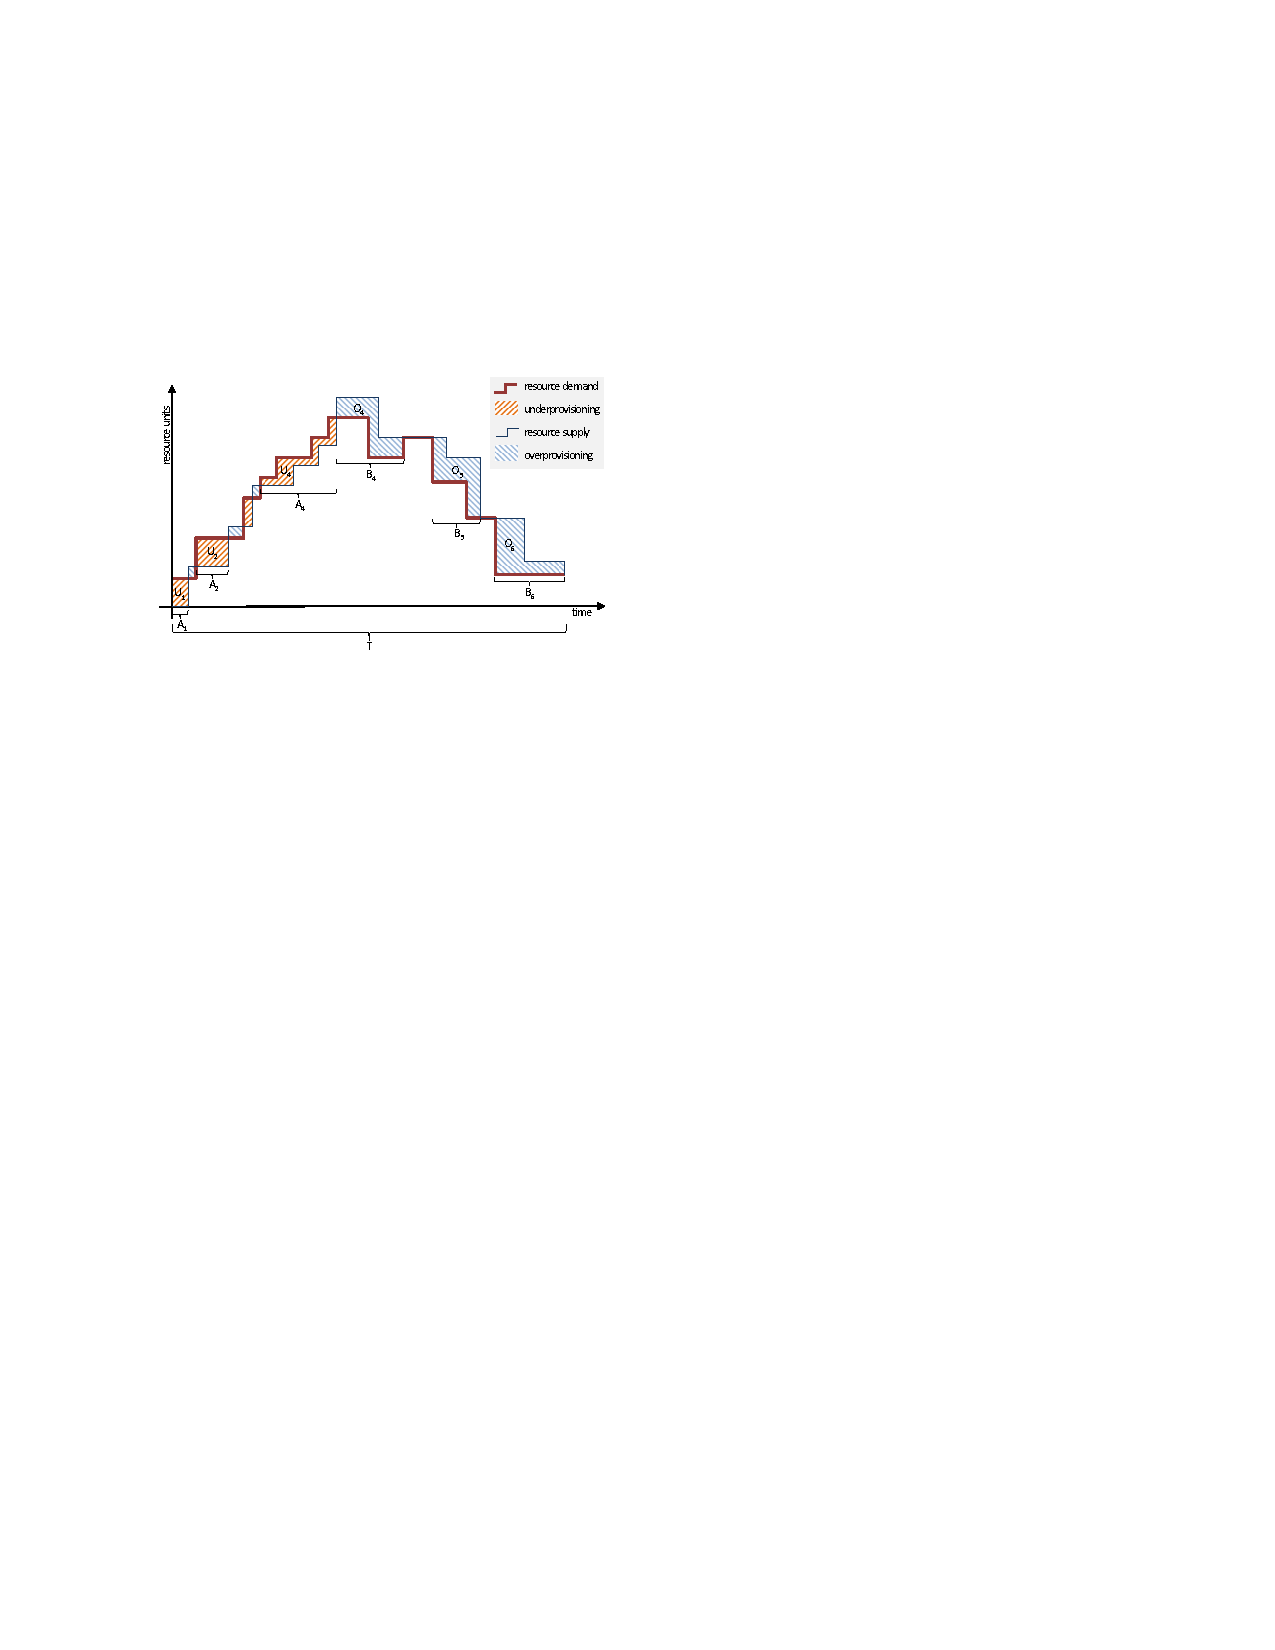
\includegraphics[clip, width=\textwidth]{images/workload}
  \end{figure}
\end{frame}

\begin{frame}
\begin{figure}
\tikzstyle{every path}=[line width=1pt, color=orange, text=white]
\def\firstcircle{(-2.85,0) circle (1.5cm)}
\def\secondcircle{(0,2.85) circle (1.5cm)}
\def\thirdcircle{(2.85,0) circle (1.5cm)}
\def\bigcircle{(0,1) ellipse (5.5cm and 3.5cm)}
\begin{tikzpicture}
    \begin{scope}[shift={(3cm,-5cm)}]
        \visible<2->{\fill[black!70] \bigcircle;}
        \fill[black!60] \firstcircle;
        \fill[black!60] \secondcircle;
        \fill[black!60] \thirdcircle;
        \visible<2->{\draw \bigcircle node [below] {\Large Elasticity};}
        \draw \firstcircle node {\Large Speed};
        \draw \secondcircle node {\Large Scalability};
        \draw \thirdcircle node {\Large Precision};
    \end{scope}
\end{tikzpicture}
\end{figure}
\end{frame}

\begin{frame}
  \frametitle{Elasticity~\cite{herbst2013elasticity}}
  \begin{definition}
  \parbox{\linewidth}{\textbf{Elasticity} is the degree to which a system is able to adapt to workload changes by provisioning and de-provisioning resources in an autonomic manner, such that at each point in time the available resources \textit{match} the current demand as closely as possible.}
  \end{definition}
\end{frame}

\begin{frame}
  \frametitle{Different parameters involved in elasticity~\cite{galante2012survey}}
  \includegraphics<1->[width=\textwidth]{images/elasticity2_1}\hspace*{-\textwidth}%
  \includegraphics<2->[width=\textwidth]{images/elasticity2_2}\hspace*{-\textwidth}%
  \includegraphics<3->[width=\textwidth]{images/elasticity2_3}\hspace*{-\textwidth}%
  \includegraphics<4->[width=\textwidth]{images/elasticity2_4}\hspace*{-\textwidth}%
\end{frame}


\section{When to Scale}
\begin{frame}
  \frametitle{Reaction~\cite{gulati2011cloud}}
  \begin{center}
    Set of rules (\textit{thresholds}).
  \end{center}

  \vspace*{\fill}

  \visible<2->{Different resource managements.~\cite{gulati2011cloud}}
  \begin{description}
    \item[Hierarchical]<3-> Management systems built on top of each other. E.g.\ cluster level with layer on top.
    \item[Flat]<4-> Completely decentralized management.
  \end{description}

  \vspace*{\fill}
\end{frame}

\begin{frame}
  \frametitle{Prediction~\cite{gulati2011cloud}}
  \begin{center}
    Models built through analysis, learning, queueing theory\dots
  \end{center}

  \vspace*{\fill}

  \visible<2->{Another resource managements.}
  \begin{description}
    \item[Statistical]<3-> Small scale with dynamic clusters. Repeated small scale optimizations attain large scale load and optimal placement.
  \end{description}

  \vspace*{\fill}
\end{frame}

\begin{frame}
  \frametitle{Example of an elasticity controller~\cite{moore2013coordinated}}
  \begin{center}
    Mixing reactive and predictive methods.
  \end{center}
  \pause{}
  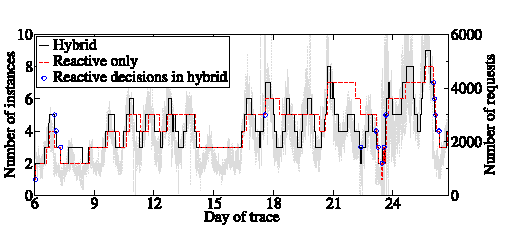
\includegraphics[width=\textwidth]{images/elasticity5}
\end{frame}


\section{How to Scale}
\begin{frame}
  \frametitle{Kinds of scaling / Mechanisms}
  \begin{description}
    \item[Horizontal]<1-> (\textit{Replication}) Adding/Removing instances (e.g.\ VMs, modules\dots).
    \item[Vertical]<2-> (\textit{Resizing}) Adding resources (e.g.\ processing, memory\dots). \textit{Not always available.}
    \item[Migration]<3-> (\textit{Scaling Out}) Transferring a VM from one physical server to another one.
  \end{description}
\end{frame}

\begin{frame}
  \frametitle{Configurations \& Transitions}
  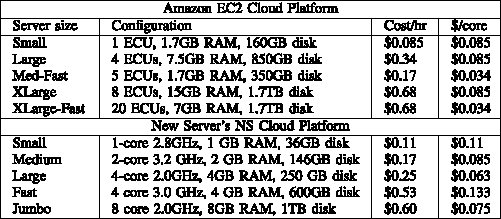
\includegraphics[width=\textwidth]{images/elasticity4_config}
  \vspace*{\fill}
  There is also cost for transition.
\end{frame}

\begin{frame}
  \frametitle{Example of a provisioning system~\cite{sharma2011cost}}
  Integer Linear Program to take into account multiple parameters.
\end{frame}

\begin{frame}
  \frametitle{Example of architecture~\cite{sharma2011cost}}
  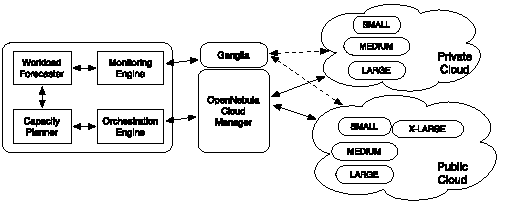
\includegraphics[width=\textwidth]{images/elasticity4_arch.pdf}
\end{frame}


\section*{Conclusion}
\begin{frame}
  \frametitle{Conclusion}
  Not there yet.
  \begin{itemize}
    \item Elements tightly coupled but studied independently.
    \item Mechanisms conceived with assuming other elements in the workflow to be perfect.
    \item Overhead can be a problem (frequency, decomposition, failures\dots).
  \end{itemize}
\end{frame}


\appendix
\section*{References}
\begin{frame}[allowframebreaks]{References}
  \bibliography{bib}
  \bibliographystyle{abbrv}
\end{frame}


\end{document}
